\documentclass{sig-alternate}
%\documentclass{acm_proc_article-sp}

\usepackage{cite, graphicx, subfigure, amsmath, xspace, txfonts}
%\usepackage{eurosym} 

\newcommand{\us}{\,$\muup$s\xspace}

\hyphenation{ob-ser-va-tion}
\hyphenation{pipe-li-nes}
\hyphenation{FPGAs}

% TODO anoniem maken

\begin{document}

\title{The LOFAR Correlator: \\ Implementation and Performance Analysis}

%% \numberofauthors{4}

%% \def\sharedaffiliation{%
%% \end{tabular}
%% \begin{tabular}{c}}

%% \author{
%% \alignauthor John W. Romein\\
%% \email{romein@astron.nl}
%% \alignauthor P. Chris Broekema\\
%% \email{broekema@astron.nl}
%% \alignauthor Jan David Mol\\
%% \email{mol@astron.nl}
%% \and
%% \alignauthor \hspace{1cm} \\
%% \alignauthor Rob V. van Nieuwpoort\\
%% \email{nieuwpoort@astron.nl}
%% \alignauthor \hspace{1cm} \\
%% \sharedaffiliation
%% \affaddr{ASTRON (Netherlands Institute for Radio Astronomy)}\\
%% \affaddr{Oude Hoogeveensedijk 4, 7991\ PD\ \ Dwingeloo, The Netherlands}\\
%% }

\date{}

\maketitle


\begin{abstract}
LOFAR is the first of a new generation of radio telescopes.
Rather than using expensive dishes, it forms a distributed sensor network that
combines the signals from many thousands of simple antennas.
Its revolutionary design allows observations in a frequency range that has
hardly been studied before.

This paper focuses on another novel feature: where traditional telescopes
use customized hardware, we process the data in \emph{software}. 
This dramatically increases flexibility and substantially reduces costs, but
the high processing and bandwidth requirements compel the use of a
supercomputer.
The antenna signals are centrally combined, filtered, optionally beam-formed,
and correlated by an IBM Blue Gene/P.

To meet the real-time requirements, the application is highly optimized, and
reaches exceptionally high computational and I/O efficiencies.
This allows us to use only half the planned amount of resources, \emph{and\/}
process 50\% more telescope data, significantly improving the effectiveness
of the entire telescope.
\end{abstract}


\section{Introduction}

\begin{figure}[t]
\begin{center}
\includegraphics[width=70mm]{LBA-field.jpg}
\end{center}
\caption{A field with low-band antennas (dipoles).}
\label{fig:lba-field}
\end{figure}

LOFAR is an acronym for \emph{\textbf{LO}w \textbf{F}requency \textbf{AR}ray},
an aperture array radio telescope operating in the 10 to 250~MHz frequency
range.
It is the first of a new generation of radio telescopes, that breaks with
the concepts of traditional telescopes in several ways.
Rather than using large, expensive dishes, LOFAR uses many thousands of
simple antennas that have no movable parts~\cite{Butcher:04,deVos:09}, see Figure~\ref{fig:lba-field}.
Essentially, it is a distributed sensor network that monitors the sky
and combines all signals centrally.
This concept requires much more signal processing, but the additional costs
of silicon are easily offset by cost savings in steel that would be needed for dishes.
Moreover, LOFAR can observe the sky in many directions concurrently and
switch directions instantaneously. 
In several ways, LOFAR will be the largest telescope of the world, 
and will enable groundbreaking research in several areas of astronomy and particle
physics~\cite{Bruyn:02}. The different goals and observation types require
several different processing pipelines, however.

Another novelty is the elaborate use of \emph{software\/} to process
the telescope data in real time. 
Previous generations of telescopes depended on custom-made hardware
because of the high data rates and processing requirements.
However, the desire for a flexible and reconfigurable instrument with
different processing pipelines for different observation types demands a
software solution.
The availability of sufficiently powerful supercomputers allows this.
We have to perform all processing in real time,
since the data streams simply are too large to store.

\begin{figure*}
\begin{minipage}[b]{11cm}
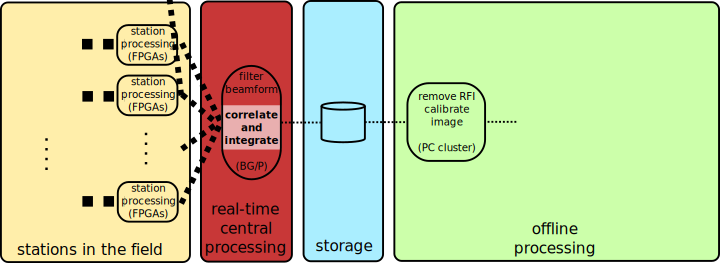
\includegraphics[width=11cm]{lofar-overview.pdf}
\caption{A simplified overview of the LOFAR processing.}
\label{fig:lofar-overview}
\end{minipage}
\hfill
\begin{minipage}[b]{56mm}
\includegraphics[width=\columnwidth]{map.jpg}
\caption{Possible LOFAR layout.}
\label{fig:map}
\end{minipage}
\end{figure*}

The most common mode of operation for LOFAR is the 
\emph{standard imaging pipeline}, which is used to generate sky images.
This mode filters and correlates the data sent by the stations.
This paper describes the implementation and
performance characteristics of the real-time part of this pipeline on an IBM Blue Gene/P (BG/P)
supercomputer.
We present a highly-optimized implementation that achieves very high
computational performance: the correlator sustains 96\% of the theoretical
floating-point peak performance during the computational phase.
%The \emph{Epoch of Reionization (EoR)\/} pipeline should detect the faint,
%very first sky objects.
%It is a similar pipeline, but with even higher computational demands, due to
%the increased amount of concurrent observation directions.
Several \emph{pulsar pipelines\/} are being developed as well, that either
search large sky regions to find unknown pulsars or, once found, sensitively
observe their characteristics.
The pipelines share common components, shortening their development time. 
The software also supports multiple concurrent observations, even of different
types.

The receivers produce hundreds of gigabits per second.
To handle the high data rate,
we use the BG/P in an unconventional way: we run
\emph{application\/} software on the so-called I/O~nodes to pre-process and
post-process data that are further handled on the compute nodes.
This yields an efficient system and substantially saved us on
costs~\cite{Iskra:08}.
Additionally, we developed a low-overhead network protocol~\cite{Romein:09a}
for communication between I/O~nodes and compute nodes, since we were not able
to achieve the required internal input and output data rates with the standard
network software.

In earlier work~\cite{Romein:06}, we presented an initial prototype
implementation of the LOFAR processing on our previous platform, the
Blue Gene/L.  The work presented in this paper differs in several
important ways.  First, we have now implemented the complete I/O path:
from the LOFAR stations in the field to the Blue Gene/P, 
from the IO~nodes to the compute nodes, the internal
data transpose, and finally the transfer 
to the storage cluster. In contrast, in~\cite{Romein:06}
we focused only on computing, and not on I/O.
Second, we now have a fully functional \emph{real time} processing pipeline
for the most important standard imaging mode, and prototypes for other
pipelines, showing the flexibility of our design.  Finally, for the
first time, we perform a scalability analysis, proving that we can 
support the requirements of the full LOFAR instrument, both in
terms of computing and I/O, in real time. In fact, we even surpass the
requirements.

This paper is structured as follows.
We mention related work in Section~\ref{sec:related-work}.
In Section~\ref{sec:overview}, we give an overview of the LOFAR telescope.
Then, in Section~\ref{sec:BG/P}, we describe the hardware characteristics of
the BG/P.
Next, we explain how we process the telescope data on the BG/P,
(Section~\ref{sec:processing}), focusing on the processing on the I/O~nodes
(Section~\ref{sec:IONProc}) and compute nodes (Section~\ref{sec:CNProc}).
Section~\ref{sec:performance} extensively discusses performance results.
In Section~\ref{sec:results}, we briefly illustrate the astronomical results
of the correlator output.
Finally, we discuss, conclude, and describe future work in
Section~\ref{sec:conclusions}.



\section{Related Work}
\label{sec:related-work}

%LOFAR is not the only radio telescope of which the data are processed in software. In fact,
%in the 1960s, several observatories~\cite{Bare:67,Moran:67} recorded their input on high-speed tapes
%and processed it on IBM 360 mainframes. However, as the volume of the data increased, the mainframes were no longer capable of processing the data in an acceptable amount of time, and custom hardware had to be used instead.

%Due to the massive increase in processing power since the 1960s, software processing of telescope
%data is once again feasible. Several efforts to do so have been started. However, to the best of our knowledge,
%LOFAR is the only system capable of processing high data rates from a large number of stations at
%real time.

On our previous platform, the BG/L, we were dissatisfied with
the I/O model and its performance.  This led to a joint effort with 
Argonne national lab to redesign the entire network software infrastructure, and resulted in a
new environment called {\em ZOID\/}~\cite{Iskra:08}.  ZOID does not
only yield better performance, but it is much more flexible, since it
allows application code to be run on the I/O~nodes.  
The standard BG/P
software infrastructure is a major improvement over the BG/L, since it
now incorporates several of ZOID's key ideas (e.g., that of running
application code on the I/O~nodes).  Therefore, we do not have to use
ZOID on the BG/P anymore.  Nevertheless, the achieved performance of the
collective network that we use to send LOFAR data from the I/O~nodes
to the compute~nodes still is unsatisfactory.  We therefore developed
our own high-performance low-overhead protocol, called FCNP.  We
describe FCNP in~\cite{Romein:09a}, but summarize the relevant features in
Section~\ref{sec:input-handling}.

%Zoid werk op ZeptoOS, kan torus niet 
%gebruiken op compute nodes, is essentieel voor ons (voor transpose).
% applicatie kan ZOID crashen. Met fcnp kan dat niet
% Rob: te veel detail hier denk ik.

The idea to implement a correlator in software has been adopted by
others as well.  However, the LOFAR correlator is the only system
capable of processing a large number of inputs at high data rates in
real time.  Other systems handle only a few inputs, handle limited
data rates, or do not run in real time.

Deller et al.~\cite{Deller:07} have developed the DiFX distributed
software correlator, which is to be deployed on a cluster of PCs.
Due to the use of commodity hardware, both their communication and
computational capabilities are substantially lower than those available in
our Blue Gene/P.
%As a result, they cannot handle the width and number of input streams that we
%process in LOFAR.
The real-time data processing of the Murchison Widefield Array (MWA) telescope
is implemented partially in software.
However, their correlator, computationally the most demanding part of the
processing pipeline, is not implemented in software, but on 
FPGAs~\cite{Ord:08}.
Finally, the Joint Institute for VLBI in Europe (JIVE) develops a new software
correlator for e-VLBI observations, but is not capable of processing telescope
data in real time~\cite{Kruithof:08}, even though the title of their paper suggests
otherwise.

In another paper, we compare the efficiency of five many-core
architectures (GPUs from Nvidia and ATI, the Cell/B.E., the Blue Gene/P,
and the Intel Core~i7) for correlation purposes~\cite{Nieuwpoort:09}.



\section{The LOFAR Telescope}
\label{sec:overview}

LOFAR is driven by the astronomical community, that needs a new instrument
to study an extensive amount of new science cases.
Five key science projects have been defined.
First, we expect to see the \emph{Epoch of Reionization\/} (EoR), the time
that the first star galaxies and quasars were formed.
%The 1.42~GHz emission line of hydrogen is expected to be
%red-shifted into the LOFAR sensitivity range.
Second, LOFAR offers a unique possibility in particle astrophysics for
studying the origin of high-energy
% ($10^{15}$--$10^{20.5}$~eV)
\emph{cosmic rays}.
Neither the source, nor the physical process that accelerates such particles
is known.
Third, LOFAR's ability to continuously monitor a large fraction of the sky
makes it uniquely suited to find new \emph{pulsars} and to study \emph{transient sources}.
Since LOFAR has no moving parts, it can instantaneously switch focus to
some galactic event.
Fourth, \emph{Deep Extragalactic Surveys\/} will be carried out to find the
most distant radio galaxies and study star-forming galaxies.
Fifth, LOFAR will be capable of observing the so far unexplored radio
waves emitted by \emph{cosmic magnetic fields}.
For a more extensive description of the astronomical aspects of the LOFAR
system, see De Bruyn et.~al.~\cite{Bruyn:02}.

A global overview of the LOFAR instrument is given in
Figure~\ref{fig:lofar-overview}. LOFAR uses two different types of
antennas: the Low-Band Antennas (LBA) for the 10--80~MHz frequency
range and High-Band Antennas (HBA) for the 110--250~MHz band.
FM radio transmissions make the in-between range unsuitable for observations.
Figure~\ref{fig:lba-field} shows a field with LBAs. Each
LBA consists of one dipole per polarization, while each HBA is
organized as a tile combining 16 antenna elements. All
antennas are dual polarized.

LOFAR's antennas are structured in a hierarchical way to limit the
costs of data transport and processing. Tens of thousands of antennas are
necessary to obtain sufficient sensitivity. The antennas are
distributed over a large area to achieve a high angular resolution.
However, combining the data of all individual antennas centrally would
require too much network bandwidth and would result in excessive
computational requirements. Therefore, multiple antennas are grouped
to form a \emph{station}.
The signals of the receivers are combined locally, within the station, using FPGAs.

Geographically, LOFAR consists of a compact core area that contains
about 50\% of the stations, and a number of
remote stations (See Figure~\ref{fig:map}).  The heart of LOFAR will
be installed in the Northern part of the Netherlands.  The stations
are roughly distributed along five log-spiral arms with a diameter of
hundreds of kilometers. 
%The station fields are centrally condensed,
%following a logarithmic distribution.  
Additionally, eight to fifteen European stations will or have been built,
extending the maximum distance to roughly 1000~km.
The longer baselines (distance between two stations) allows observations with high angular resolution,
but limits the Field-of-View; therefore the European stations will not be
used for all observations.
%In the past several years we have deployed a number of prototype antennas,
The roll-out of the stations is currently in progress.

Each station is equipped with 48--96 LBAs and 48--96 HBA tiles. 
A station also features a cabinet where initial processing is done.
Typical operations that are performed here include analog-to-digital
conversion, filtering, frequency selection, and combination of the signals
from the different receivers.
One of the distinctive properties of LOFAR is that the receivers are
omni-directional, and that multiple, concurrent observation directions are
supported.
Since observing the sky in all frequencies and all directions at the same time
would result in an unmanageable output data rate, the observer selects a
limited number of directions and frequencies, called \emph{subbands}.

The station data are transported to the central processing location 
via a Wide-Area Network (WAN), using dedicated light paths.
We use UDP for data transport, since we can easily tolerate some data loss.
We do not use a reliable protocol such as TCP, because this significantly
complicates the programming of the station FPGAs, due to buffering, flow control,
retransmission, and real-time issues.

The UDP packets contain samples, where a sample is a complex number
that represents the amplitude and phase of a signal at a particular
time.  A sample is encoded by a $2\times4$, $2\times8$, or $2\times16$-bit
complex integer. Data can be invalid for various reasons, such as
lost network packets or \emph{Radio Frequency Interference\/} (RFI, e.g.,
caused by TV transmitters).
Throughout the entire processing chain, we maintain which
data is marked as invalid, so that eventual images are not distorted by
bad data.  

This paper focuses on the real-time, central processing of LOFAR data
on an IBM Blue Gene/P supercomputer, and in particular on the
standard-imaging mode.  We chose the BG/P as the central processing
platform, instead of, for instance, a cluster with a fast local
interconnect, for several reasons.
First, the BG/P has excellent hardware
support for complex numbers, a feature that is of key
importance for signal-processing applications, but is lacking in
general-purpose architectures. 
Moreover, the BG/P has a very high
memory bandwidth per operation. This leads to superior performance for our
data-intensive applications, compared to other platforms~\cite{Nieuwpoort:09}.
In addition, the BG/P provides a high-speed 3D-torus network that can
effectively implement a data-transpose that is crucial for our
application, at the bandwidth we require (see Section~\ref{all-to-all}). 
Finally, the BG/P is a power-efficient supercomputer.
Electrical power costs form a large part of the operational costs for
the LOFAR instrument.  At the time of purchase, the BG/P was the highest-ranking 
system on the green500 list for energy
efficient supercomputers (see www.green500.org). 

Our pipeline on the BG/P filters the data, and splits the subbands in narrower frequency bands called
\emph{channels}, which allow for more accurate RFI removal.
In addition, we perform phase shift and bandpass corrections.
Finally, the signals from all stations are optionally beam-formed,
correlated and forwarded to a storage cluster, where results can be
kept for several days. 
After an observation has finished, further processing is done off-line, on
commodity cluster hardware. 
%First, the \emph{flagger\/} uses an RFI detection algorithm to remove bad data.
%Then, the results are calibrated for instrumental and environmental effects and
%for sky source parameters (e.g., position, flux)~\cite{Nijboer:07}.
%An imaging algorithm creates an image of the observed source(s).
Despite considerable computational challenges, the scope of this paper does not cover
the off-line processing.

Prototypes of other observation modes, used to find and observe
pulsars, are functional, but are not optimized for performance yet.
Hence, we do not discuss the pulsar modes in this paper.
However, the presence of multiple observation modes demonstrates the
flexibility of a \emph{software\/} solution.
%More observation modes will be implemented in the future.




\section{The Blue Gene/P}
\label{sec:BG/P}

Initially, LOFAR used a 6-rack IBM Blue Gene/L supercomputer for real-time
processing of the station data.
We recently replaced the system by an equally powerful 2.5-rack Blue Gene/P.
%The consequences of this upgrade are described in Section~\ref{sec:upgrade}.
Below, we describe the key features of the Blue Gene/P.
More information can be found elsewhere~\cite{IBM:08}.

Our system contains 10,880 processor cores that provide 37.0 TFLOPS peak
processing power.
% (including I/O~nodes).
%The system is built using SoC (System-on-a-Chip) technology that integrates
%all processing and networking functionality on a single die.
One chip contains four PowerPC~450 cores, running at a modest 850~MHz clock
speed to reduce power consumption and increase package density.
Each core has two Floating-Point Units (FPU) that provide support for
operations on complex numbers.
%A core can sustain two fused multiply-adds per cycle.
%The four cores share 2~GiB of main memory.
%% Although a node can run in \emph{SMP mode}, we run the application in
%% \emph{virtual node mode}, where the processor and memory of a node are split
%% into four independent, virtual machines.
%% This simplifies programming, since this allows single-threaded processing
%% on the compute cores.  % TODO: tree is shared resource; mention?
The compute nodes run a fast, simple, single-process kernel
\emph{(Compute Node Kernel, CNK)},

%% \begin{figure}[b]
%% \includegraphics[width=\columnwidth]{pset.pdf}
%% \caption{A pset.}
%% \label{fig:pset}
%% \end{figure}

The BG/P contains several networks.
A fast \emph{3-dimensional torus\/} connects all compute nodes and is used
for point-to-point and all-to-all communications.
Unlike the BG/L, the torus uses DMA to offload the CPUs and allows
asynchronous communication.
The \emph{collective network\/} is used for MPI collective operations,
but also for external communication.
%A \emph{global interrupt network\/} provides support for fast barriers.
Additional networks exist for fast barriers, initialization, diagnostics, and debugging.

Each compute node is connected to an I/O~node via the collective network.
%(see Figure~\ref{fig:pset}).
An I/O~node uses the same hardware as a compute node, but has its 10 Gb/s Ethernet
interface connected and runs another operating system (a modified Linux kernel).
%Since our application demands high bandwidths, our system is configured with
%the maximum number of 1~I/O~node per 16~compute nodes (64~cores).
The group of one I/O~node and the compute nodes that are connected to it (16 in our case),
is called a \emph{pset}.
Our system has 160~psets in total, 64 per rack.
Normally, the I/O~node is used as a black box that provides transparent
communication from the compute nodes to external systems.
%: all I/O-related
%system calls on the compute nodes are forwarded to a daemon that runs
%on the I/O~node and performs the real operation.
In Section~\ref{sec:IONProc}, we show that it is much more
efficient to run part of the application software on the I/O~node.


\section{LOFAR Processing}
\label{sec:processing}

\begin{figure}[ht]
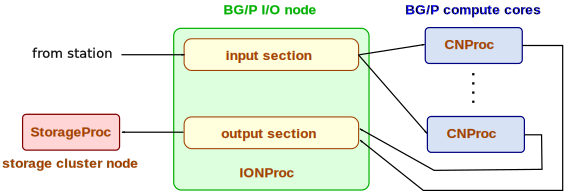
\includegraphics[width=\columnwidth]{processing-overview.pdf}
\caption{Simplified data flow diagram for the central processing pipeline.}
\label{fig:processing}
\end{figure}

The LOFAR station data are centrally processed in real time by a collection
of three distributed applications.
These applications run on different platforms:
the Blue Gene/P \emph{I/O nodes}, the Blue Gene/P \emph{compute nodes}, and on
external (PC-like) \emph{storage nodes}.
Figure~\ref{fig:processing} shows how the data flows through the entire
processing chain.
The first application, \emph{IONProc}, runs on the Blue Gene/P I/O nodes.
Its main tasks are to receive the station UDP data, to buffer the data
for up to 2.5~seconds, and to forward it to the compute nodes in the pset.
The second application, called \emph{CNProc}, runs on the Blue Gene/P compute
nodes, where the compute-intensive processing takes place.
The main tasks are to reorder the data across the compute nodes over the
internal torus network, to filter the data, and to correlate or beam-form
the filtered data.
The resulting data are then sent back to the I/O-node application, that
collects the data from the compute nodes and
sends the data to the storage nodes.
This is where the third application (StorageProc) runs.
The storage nodes are PC-like systems with large disks.
The storage application collects the data from the I/O~nodes and writes the
data to disk.


\section{I/O-node Processing}
\label{sec:IONProc}

\begin{figure}[t]
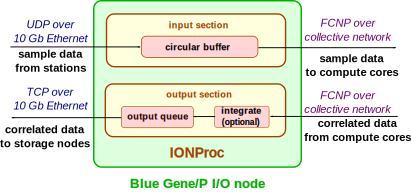
\includegraphics[width=\columnwidth]{ION-processing.pdf}
\caption{Simplified data flow diagram for the I/O nodes.}
\label{fig:ion-processing}
\end{figure}

We use the Blue Gene in an innovative way, by running application software
on the I/O~nodes.
On the Blue Gene/L, this required rewriting major parts of the system
software~\cite{Iskra:08}, but this idea is much better supported on the
Blue Gene/P.

We run one multi-threaded process on each I/O~node that takes care of two
tasks: the handling of input and the handling of output (see
Figure~\ref{fig:ion-processing}).
The \emph{input section\/} deals with receipt of UDP station data, buffering,
and forwarding to the compute nodes.
The \emph{output section\/} collects outgoing result data from the compute
nodes, optionally integrates the data over multiple seconds in time, and
forwards the data to storage.
An I/O node may run both sections, only one of them, or none at all, depending
on the configuration.
Both tasks are described in detail below.


\subsection{The Input Section}
\label{sec:input-handling}

The LOFAR stations send UDP packets with sampled data over a
dedicated Wide-Area Network to a BG/P I/O~node.
The data are received by the \emph{input section}.
To simplify the implementation of the correlator, there is a one-to-one
mapping between stations and I/O~nodes, so that one I/O~node receives all
data from a single station.
However, handling the full 3.1~Gb/s data rate of a station on a relatively
slow CPU is quite a challenge, since sufficient processing time must be left
for handling output as well.
Note that an I/O~node does not run the input section if it is not
connected to a station.

The input section receives the UDP packets, taking care of out-of-order,
duplicated, and lost packets.
At each station, four of the FPGAs send data to their associated I/O~node,
each FPGA to a different UDP port.
The I/O~node runs four ``input'' threads, one thread per socket.
Multiple threads are necessary, since we have to utilize multiple cores; a single core is too slow to receive all
data.
Together, the threads receive a total of 48,828~packets per second.

The samples from the received UDP packets are copied into a circular buffer that
holds the most recent 2.5~seconds of data.
The buffer serves three purposes.
First, it is used to synchronize the stations, since the travel times over
the WAN are higher for the remote stations than for the central stations.
Second, the buffer prevents data loss due to small variations in processing
times of the remainder of the pipeline.
Third, the buffer is used to artificially delay the stream of samples,
as we will explain in Section~\ref{sec:signal-processing}.
The buffer is limited by the small memory size, but due to good real-time
behavior of the application, 2.5~seconds is sufficient.

Another thread reads data from the circular buffer and sends the data to
the compute nodes for further processing. 
It sends data in large bursts that contain approximately one second worth of samples.
Unfortunately, existing network software did not provide sufficient bandwidth
and consumed too much CPU time.
We therefore developed \emph{FCNP (Fast Collective-Network Protocol)}, a 
network library for high-bandwidth communication between the I/O~nodes and the
compute nodes~\cite{Romein:09a}.
FCNP achieves link-speed bandwidths for large messages, due to
its low overhead.
The data are sent directly from the circular buffer without additional copying.
In contrast to the UDP receive, one thread is sufficient to obtain the
required throughput, thanks to the low processing overhead of FCNP.

The correlator typically processes in real time, but can also correlate
pre-recorded data off-line, frequently used for experimental observations.
When processing in real time, the NTP-synchronized wall-clock time
is used to trigger the sending of a new block of data.
A block of data containing samples from time $t_1$ to $t_2$ are sent some 
hundreds of milliseconds (the WAN delay plus a safe margin) after $t_2$,
whether or not all data were actually received from the station.
This assures real-time continuation of the correlator and
provides fault-tolerance against a failing station or WAN link.
In practice, this method causes hardly any data loss.
When processing off-line, the input is read from file or TCP socket rather
than a UDP socket.
In off-line mode we do not use the wall-clock time as
trigger, but we synchronize the threads that read and write the circular
buffer differently to prevent them from overtaking each other.


\subsection{The Output Section}

The bulk of the signal processing is done on the compute nodes, on which we
elaborate in Section~\ref{sec:CNProc}.
The resulting output data are sent back to the I/O~node.
The second major task of the I/O-node application is the \emph{output section},
that handles output data.
This task consists of four operations.

First, the data are received from the compute nodes, also using FCNP.
Second, the data are optionally added to previously received data from other
compute nodes in the pset, if integration over multiple seconds is desired.
Third, the (possibly integrated) output is queued in a buffer.
Fourth, another thread asynchronously dequeues the data and sends them to
a storage node, using TCP.

The queue improves real-time behavior and increases fault tolerance, since
it handles data on a best-effort basis.
If, for any reason, the data are not sent quickly enough to the storage node
(e.g., due to a disk or network failure), the queue fills up and subsequent
data are simply discarded until space is available.
This mechanism is important to keep the correlator running in real
time: it is much better to lose a small part of the data than to stall the
entire correlator and lose \emph{all\/} data.
In practice, under normal circumstances, no data are lost here.


\begin{figure*}[ht]
\begin{center}
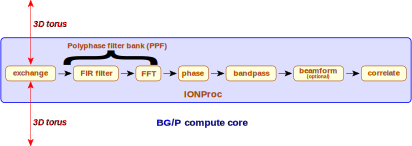
\includegraphics[width=.8\textwidth]{CN-processing.pdf}
\end{center}
\caption{Simplified data flow diagram for the compute nodes.}
\label{fig:cn-processing}
\end{figure*}

\subsection{Optimizations}

Processing power on the I/O~nodes is a scarce resource, and most observation
modes are I/O bound.
We performed many optimizations to improve processing speed.
An important improvement was to implement the function that copies data from a
received UDP packet to the circular buffer in assembly.
This way, we can exploit the efficient 16-byte load and
store instructions, which are unknown to the C++ compiler.
Unfortunately, the copy itself cannot be avoided, since an UDP packet contains
data of many frequency subbands that must be stored to different memory
locations.

Despite this optimization, we initially found that copying was very slow.
This was caused by the fact that the PowerPC~450 cannot handle
TLB\footnote{Translation Look-aside Buffer: a cache that caches
virtual-to-physical address mappings --- indispensable for efficient virtual
memory.} misses in hardware, but generates an interrupt and handles the fault
in software.
This is not a problem on the compute nodes, where the compute-node kernels 
map all memory using a few large pages, so that TLB misses do not occur.
However, the I/O~nodes run a Linux kernel that typically uses a page size of
4~KiB, generating a huge number of TLB-miss interrupts.

To avoid the interrupts, we use a modified ZeptoOS (Linux-based)
kernel\cite{Yoshii:09}.
It allows a process to map 1.5~GiB (out of 2~GiB) of physical memory in its
virtual memory map, using six fixed mappings of 256~MiB that are never evicted
from the TLB.
Hence, this memory does not generate TLB misses.
The remainder of the memory is used for normal, paged operation.
The application uses the fast memory for the circular buffer and for the
output queues.
Copying data from received UDP packets to the input buffer is up to five times
faster than when using paged memory.

To achieve good real-time behavior, we found that it is of utmost importance
to carefully manage thread priorities using the Linux real-time scheduler.
Since the compute nodes must always be able to proceed, they must be fed with
data without delays.
Therefore, the thread that sends data from the circular buffer to the
compute nodes runs at the highest priority, and is scheduled as soon as the
wall-clock time triggers.
The thread that reads results from the compute nodes is almost as
important, since compute nodes will not accept new work before the previous
results were read by the I/O~node.
Other threads, such as the threads that read UDP data, and the threads that
send data from the output queues are less important: if they would ever
fail to meet a real-time deadline, only a small amount of data is lost.
In practice, under normal circumstances, this rarely happens
(see Section~\ref{sec:ION-performance}).

%\begin{figure}
%\includegraphics[width=\columnwidth]{ion-performance.pdf}
%\caption{Performance breakdown of I/O-node processing.  See text.}
%\label{fig:ion-performance}
%\end{figure}



\section{Compute-node Processing}
\label{sec:CNProc}

The bulk of the signal-processing computations take place on the compute nodes.
In this section, we continue describing the processing pipeline depicted in
Figure~\ref{fig:processing}. 
We explain how the work is scheduled over the compute nodes, how the data are
received from the I/O~nodes, how the data are exchanged between other compute
nodes, what signal processing takes place, and which optimizations were
implemented.
The compute node pipeline is shown in more detail in
Figure~\ref{fig:cn-processing}.


\subsection{Scheduling}

\begin{figure}[ht]
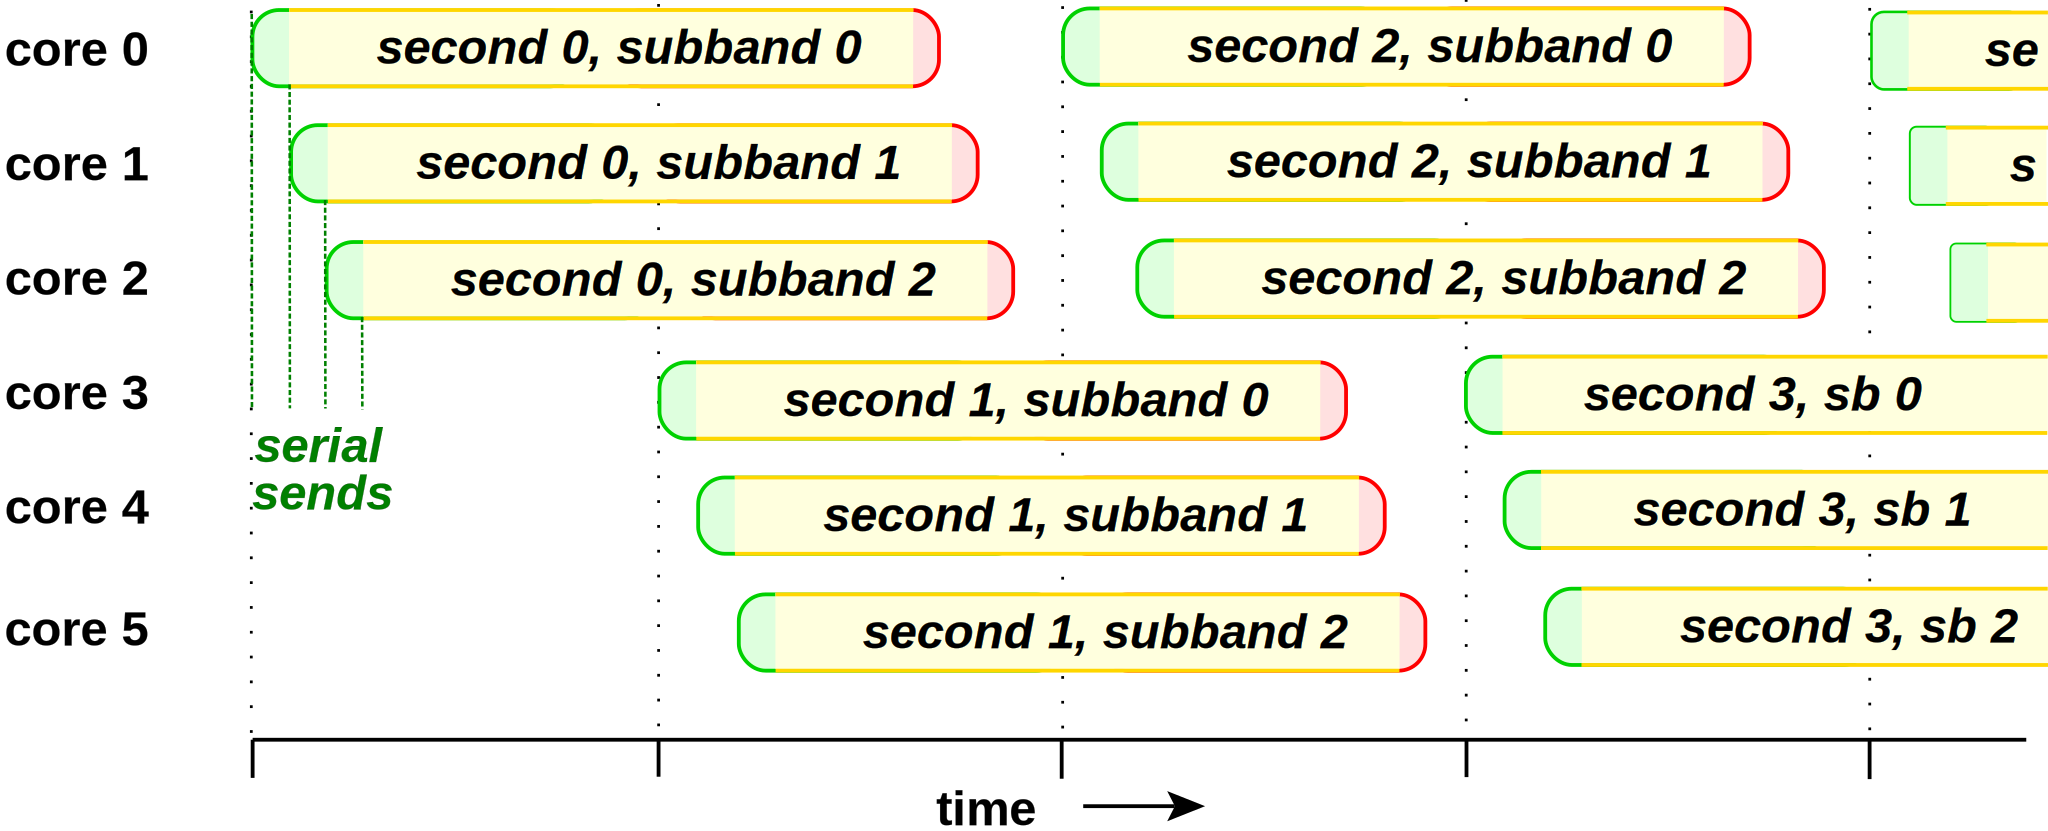
\includegraphics[width=\columnwidth]{round-robin.pdf}
\caption{Round-robin work distribution.}
\label{fig:round-robin}
\end{figure}

The I/O~node chops the data stream that comes from the station into chunks of
one frequency subband and approximately one second of time.
Such a chunk is the unit of data that is sent to the compute node for further
processing.
Since processing a chunk typically takes much longer than one second,
the chunks are round-robin distributed over a group of processor cores,
as illustrated by Figure~\ref{fig:round-robin}.
Subsequent chunks are processed by different processor cores.
A core must finish its work before it is time to process the next chunk.
A core first receives data from the I/O~node (green in the figure),
processes them (yellow), sends back the results (red), and idles until the
I/O~node sends new data.

For simplicity, Figure~\ref{fig:round-robin} shows the processing of
three subbands on six cores.
In reality, scheduling is more complex.
The subbands that must be processed are first (more or less) evenly divided
over the psets.
Typically, a pset is responsible for a fixed set of four to sixteen subbands.
Then, the subbands are round-robin scheduled over the 64~cores \emph{within the
pset}.
For example, if a pset processes six subbands, every second, the next six
cores are scheduled and each of the cores will process one subband.
In this example, the available time to process one subband is ten seconds
($\lfloor\frac{64}{6}\rfloor$).
Since consecutive chunks of a particular subband are always processed by cores
within the same pset, the output for the subband is always sent via the same
I/O~node.
This greatly simplifies communication to the storage nodes and avoids
all-to-all communication over the 10~GbE switches.
If we would have scheduled all subbands over one large pool of compute cores
rather than psets, additional communication over the torus to reroute the
output would have been necessary.
On the BG/L, this could not be implemented efficiently due to the
inability to asynchronously communicate data using a DMA engine; on the
BG/P, it unnecessarily increases torus communication.


\subsection{All-to-All Data Exchange}
\label{all-to-all}

The compute nodes perform several operations on the data, as shown in
Figure~\ref{fig:cn-processing}.
The very first step is to exchange data with another group of processor cores.
This is necessary, because an I/O~node receives all frequency subbands from one
station, but the correlator requires one frequency subband from all
stations (we explain this in more detail below).
The data exchange is challenging, since it involves hundreds of gigabits per
second.
Unfortunately, an I/O~node cannot send the data directly from the circular
buffer to the compute core that will process the data, since the I/O~node is
only connected to the compute nodes in its own pset.
The data are thus first sent over the collective network from the I/O~node to
a compute node and then over the 3-D~torus network.
The torus provides high bandwidth and switches packets efficiently.

\begin{figure}[ht]
\begin{center}
\includegraphics[width=25mm]{colinear.pdf}
\end{center}
\vspace{-0.5cm}
\caption{The bandwidth between colinear nodes is lower than between
non-colinear nodes.}
\label{fig:colinear}
\end{figure}

The torus bandwidth between colinear and coplanar nodes is lower than between
non-coplanar nodes, since non-coplanar nodes communicate over more links
(in three dimensions) simultaneously.
Figure~\ref{fig:colinear} illustrates this; the bandwidth between nodes
\textsf{A} and \textsf{B} is (in theory) three times as high as the bandwidth
between nodes \textsf{A} and \textsf{C} (in practice, it is somewhat less).
Therefore, we schedule work that needs exchange of data 
on non-coplanar cores as much as possible.
We also schedule the work so that multiple cores of the same processor do not
need to access the torus or collective network simultaneously, since these
resources are shared and simultaneous access decreases performance.
The program parts that implement the data exchange and scheduling are, in the
presence of many stations, many subbands, time slicing, round-robin core
allocation, and avoidance of resource conflicts, \emph{extremely\/}
complicated, but highly efficient.

On the BG/L, the data exchange was implemented synchronously, using
\texttt{MPI\_Alltoallv()}.
The BG/P, in contrast, uses DMA for the torus, allowing asynchronous
communication.
We re-implemented the exchange using asynchronous point-to-point
communication, that overlaps the communication over the torus network with 
the transfer from the I/O~nodes to the compute nodes, and with
the next four processing steps.
As soon as a chunk of data from one station has arrived, the core starts
processing them, up to the point that the data from \emph{all\/} stations
are required. As we will explain in the next section, this is before the beam forming 
step.


\subsection{Signal Processing}
\label{sec:signal-processing}

After the data exchange, a compute core has the samples of one subband
from all stations.
The data are processed in a number of steps, as shown in Figure~\ref{fig:cn-processing}.
We briefly describe the steps below; more details can be found elsewhere~\cite{Romein:06}.
We finish the section with some remarks on flexibility and optimizations.


\subsubsection{Data Conversion}
First, we convert the 4-bit, 8-bit, or 16-bit little-endian integer
samples to 32-bit big-endian floating point numbers.  We do this
because the Blue Gene is much better at floating-point processing than
integer processing.  Unfortunately, there is no hardware support
for integer to floating-point conversions.  We therefore use a lookup
table to convert 4-bit and 8-bit numbers, and an efficient assembly
implementation to convert 16-bit numbers.
Since the conversion increases the data size, we perform it \emph{after\/} the
data exchange.
Since the samples are at most 16-bit wide, single precision floating
point is enough for our purposes. Other telescopes use typically 2--4 bits
per sample.


\subsubsection{The Poly-Phase Filter Bank}
Next, the subband data are processed by a Poly-Phase Filter
bank (PPF) that splits a frequency subband into a number of
narrower frequency channels.  In this step, we trade time
resolution for frequency resolution: we split a subband into $N$
separate channels, but with an $N$-times lower sampling rate per channel.  With
the higher frequency resolution, we can remove RFI artifacts with a
higher accuracy later later in the pipeline.
Typically, a 195~KHz subband is split into 256~channels of 763~Hz, but the
filter supports any reasonable power-of-two number of channels for different
observation modes. 

The PPF consists of two parts. 
First, the data is filtered using Finite Impulse Response (FIR)
filters. A FIR filter simply multiplies a sample with a real weight factor, and
also adds a number of weighted samples from the past.  Since we have
to support different numbers of channels, our software automatically designs
a filter bank with the desired properties and number of channels at
run time, generating the FIR filter weights on the fly. This again
demonstrates the flexibility of a software solution.  For performance reasons, the
implementation of the filter is done in assembly.
Second, the filtered data are Fourier Transformed. We use the Blue
Gene ``Vienna'' version of FFTW~\cite{Lorenz:05} to do this. Since the
most common observation mode uses 256 channels, we optimized this case
a bit further, and manually wrote a more efficient assembly
implementation for the 256-point FFT.


\subsubsection{Phase Shift Correction}

%% \begin{figure}[ht]
%% \begin{center}
%% \includegraphics[width=2.5cm]{delay.pdf}
%% \end{center}
%% \vspace{-0.5cm}
%% \caption{The left antenna receives the wave later.}
%% \label{fig:delay}
%% \end{figure}


\begin{figure}[ht]
\begin{minipage}[b]{4cm}
\includegraphics[width=3cm]{delay.pdf}
\caption{The left antenna receives the wave later.}
\label{fig:delay}
\end{minipage}
\hfill
\begin{minipage}[b]{4cm}
\includegraphics[width=3cm]{bandpass.pdf}
\caption{Not all channels have equal signal power.}
\label{fig:bandpass}
\end{minipage}
\end{figure}

Due to the finite speed
of electromagnetic waves, the wavefront from a celestial source hits
stations at different times (see Figure~\ref{fig:delay}).  The time
difference depends on the direction of the observed source and on the
station positions, and is continuously altered by the rotation of the
earth.  Before the signals can be correlated, all station streams have
to be aligned.

Since delays can be larger than the sample period, we perform delay
compensation in two steps.  First, we correct for integer multiples of
the sample period by simply delaying the streams of station samples.
This shift is performed on the I/O~node, by moving the read
pointer of the circular buffer (see Section~\ref{sec:input-handling}).

Second, the remaining error is corrected by rotating the phase of the
signal.  The phase rotation itself costs a complex multiplication per
sample.  
%Since the phase rotation depends on the frequency, the correction
%is done after the PPF: the correction is more accurate on narrow
%frequency channels.  
The delays are computed for the begin
time and end time of a chunk, and interpolated in frequency and time
for each individual sample, with another complex multiplication.


\subsubsection{Bandpass Correction}
The bandpass correction step compensates for an artifact
introduced by a filter back that runs on the FPGAs in the stations.
This filter bank performed the initial division of the antenna signals into subbands.
Without correction, some channels have a stronger signal than others (see Figure~\ref{fig:bandpass}).
The correction is performed by multiplying each complex sample by a real,
channel-dependent value that is computed in advance.
A station cannot correct for this artifact itself, since it is only visible
in channels, not in subbands.
%We describe how the correction factors are computed in~\cite{Romein:08}.


\subsubsection{Finalizing the Asynchronous Transpose}

Up to this point in the pipeline, processing chunks from different stations can be done
independently, but from here on, the data from all stations are required.
Therefore, the asynchronous exchange ends here, before the beam forming.


\subsubsection{Beam Forming}

The beam forming step is optional, and adds the samples
from a group of stations that are close together, so that the group forms a virtual
``superstation'' with more sensitivity.
By applying an additional phase rotation (a complex multiplication), 
beam forming can also be used to select observation directions, or to
observe a large parts of the sky simultaneously.
The first is used for known pulsar and transient observations, while the latter can be 
used when searching for unknown pulsars, for instance.
The different beam forming modes are implemented, but not optimized yet.
Therefore we only mention them here to show the flexibility of a software solution, but do not include
them in the performance measurements of Section~\ref{sec:performance}.


%This step will typically be used in European observations.
%From the perspective of an international station, the baselines to the core
%stations are nearly identical.
%Treating the baselines separately makes no sense and increases the correlator
%output unnecessarily.
%Other uses of grouped, beam-formed stations are foreseen.
%% The \emph{coherent\/} way of beam forming is a special case of the beam
%% forming algorithms that are also used for pulsar and transient observations.
%% With coherent beam forming, the (phase-corrected) complex samples from
%% different stations are added.
%% The applied phase correction determines the observation direction.
%% \emph{Incoherent\/} beam forming is performed by adding the powers (amplitudes)
%% of the samples.
%% Since the phase information is lost, this mode sees a much larger part of the
%% sky, and is used to search for unknown pulsars.



\subsubsection{Correlation}

Finally, the samples from individual or grouped stations
are correlated.
The received signals from sky sources are so weak, that the antennas mainly
receive noise.
To see if there is statistical coherence in the noise, simultaneous samples of
each \emph{pair\/} of stations are correlated, by multiplying the sample of one
station with the complex conjugate of the sample of the other station.
To reduce the output size, the products are integrated, by accumulating all
products.
We accumulate 768~correlations at 763~Hz, so that the integration time is
approximately one second, the size of a chunk.
The correlator is the most time-consuming operation in the signal
processing path, because its cost grows quadratically with the number of stations.
All other steps have a lower time complexity.

%Correlation is done for each pair of stations, and for each channel separately.
%Since the correlation of station~A and~B is the complex conjugate of the
%correlation of station~B and~A, only one pair is computed.
%Stations are also autocorrelated, i.e., with themselves.
%Both polarizations of station~A are correlated with both polarizations of
%station~B, yielding correlations in XX, XY, YX, and YY directions.
%The result, a correlation, contains the combined contribution of all visible
%sky sources.
%These are disambiguated during the imaging step in the off-line processing
%pipeline.


\subsubsection{Flexibility}

We support concurrent pulsar and imaging observations, even on the
same data.  This is more efficient since the
computations in the shared components of the pipelines are done only
once. Moreover, more astronomical science can be done with a
single observation.  Additionally, in the future these pipelines can
benefit from each other.  For example, the results from
the standard imaging pipeline can be used to calibrate the data in the pulsar pipeline
in real time.

%, so that the
%pulsar pipeline can beam-form calibrated samples.
%This would not be possible without correlating the data, and would be
%particularly useful to compensate for station clock drifts, for example.


\subsubsection{Optimizations}

For optimal performance, time-critical code is written in assembly,
because the performance from compiled C++ code was by far not sufficient.
We maintain equivalent C++ reference code for testing and portability.
The assembly version hides load and instruction latencies, issues concurrent
floating point, integer, and load/store instructions,
and uses the L2 prefetch buffers in the most optimal way.
Most instructions are parallel fused multiply-adds, that sustain four
operations per cycle.

Although the FIR filters, FFTs, delay compensation, and bandpass correction
are conceptually separate, consecutive blocks, their implementations are
highly interleaved to achieve better performance.
This increases the efficiency of the L1~cache.
Also, the data are laid out in memory in such a way that they are read
consecutively as much as possible, allowing burst transfers through the
cache hierarchy.

\begin{figure}[ht]
\begin{center}
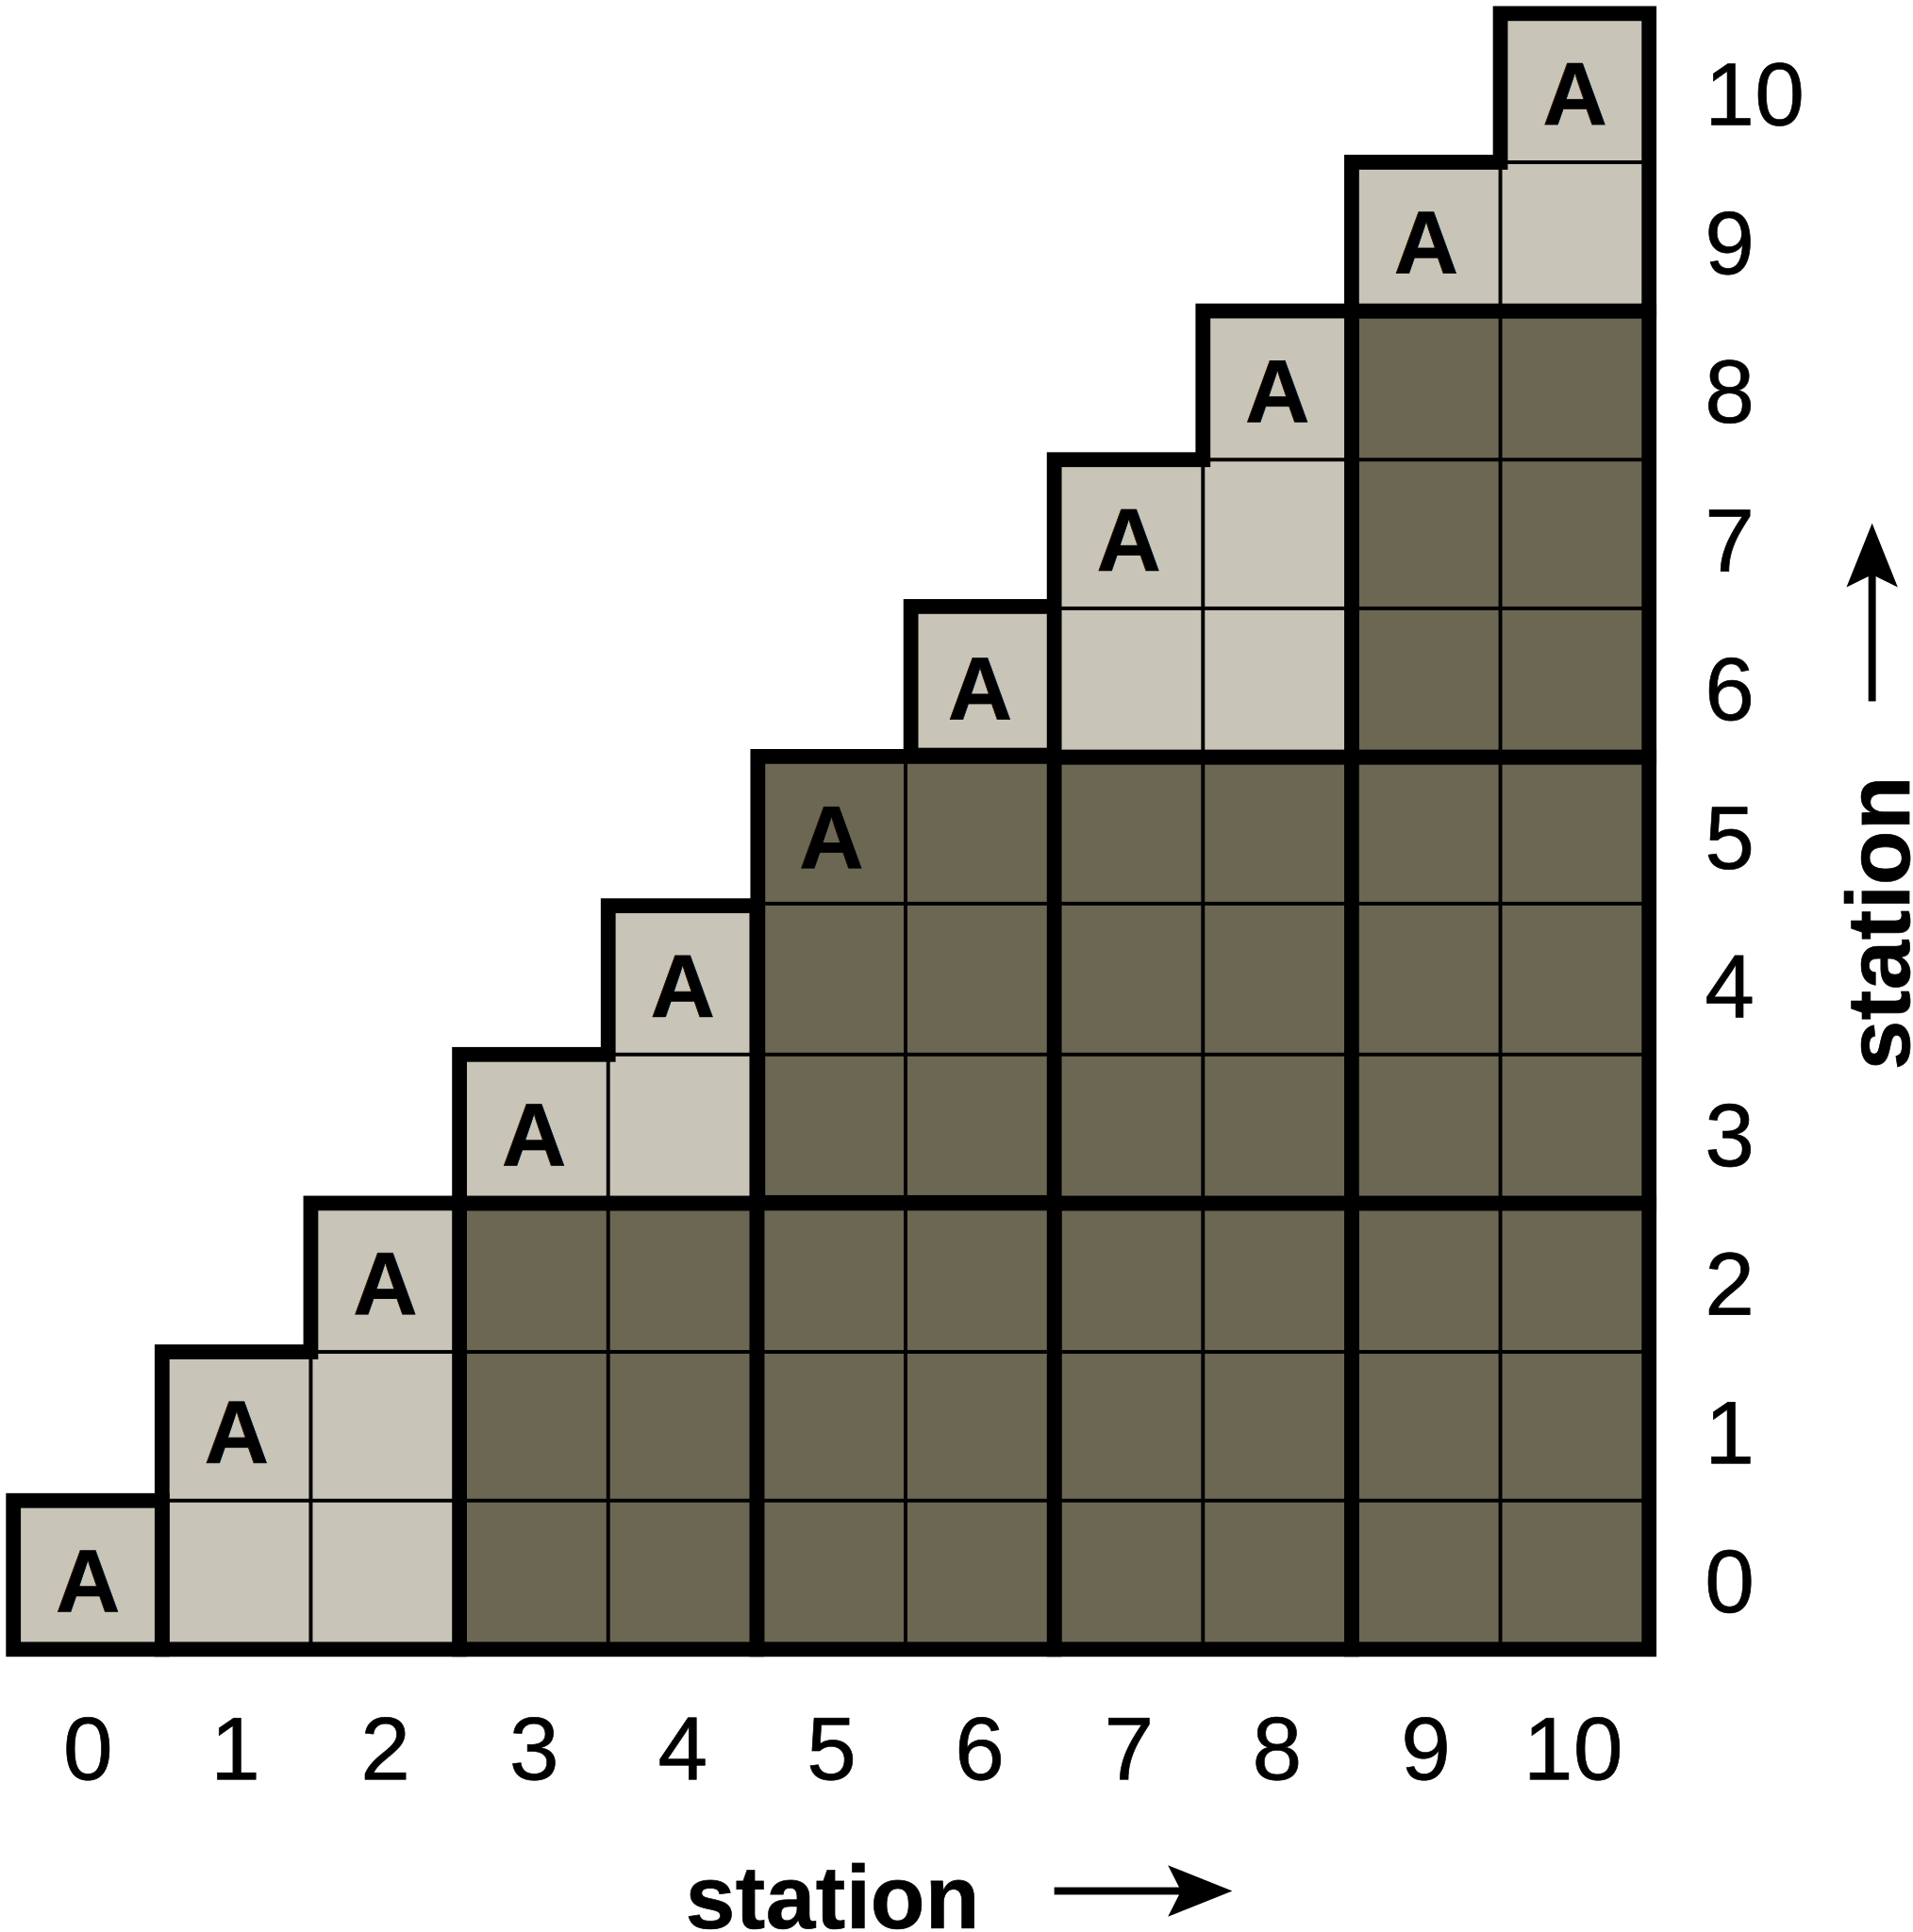
\includegraphics[width=40mm]{correlation-triangle.pdf}
\end{center}
\caption{The correlation triangle is divided into as many $2\times2$ tiles as possible.}
\label{fig:correlation-triangle}
\end{figure}

An example of an optimization that we implemented is the reduction of
memory references by the correlator~\cite{Romein:06}.
This is achieved by keeping correlations that are being integrated
in registers, and by reusing samples that are loaded from memory as often
as possible.
A sample can be used multiple times by correlating it with the samples from
multiple other stations in the same step.
For example, a sample from station~A in the X~polarization that is loaded into
a register pair can be correlated with the X~and Y~polarizations of
stations~B and~C, using it 4 times.
%In fact, it is used 8~times, since a complex multiply/accumulate requires two
%instructions.
Figure~\ref{fig:correlation-triangle} shows how we correlate multiple
stations at the same time.
Each square represents the XX, XY, YX, and YY correlations of the stations
as indicated by row and column number.
The figure is triangular, because we only compute the correlation of each
pair of stations.
The squares labeled ``\textsf{A}'' are autocorrelations, that are treated
specially since they require fewer computations.
The triangle is divided into as many $2\times2$ tiles as possible. With this size, 
the best performance is obtained.
%These $2\times2$ tiles are correlated interleaved.
For example, the lower right-hand-side rectangle correlates stations 8 and~9
with stations 0 and~1.
The X and Y samples of each of these four stations are read, requiring eight
memory load instructions (one load instruction reads a complex sample).
Computing the correlations requires 128~real operations, i.e.\ 32~instructions.
Hence, four floating-point instructions per load instruction are performed.
An unoptimized implementation would perform four times more memory accesses,
making the memory subsystem a severe bottleneck.
The interleaved correlation computations also help to hide the 5-cycle
instruction latencies of the fused multiply-add instructions, since
the correlations are independently computed.

%This is not always possible, and in those cases we try to hide the memory
%Also, many of the computations are hidden by the memory access delays that
%are the result of a transpose in main memory.

%Although the correlator (including the other signal-processing steps) is a
%typical example of a streaming-data application, the perception ``byte goes
%in, byte comes out'' is misleading.
%The data are necessarily cut into large chunks, and basically every processing
%step needs the data in another order than the previous step produced.
%This maps poorly to the memory subsystem, that is not optimized for
%non-consecutive memory accesses.
%We also found that the round-robin replacement algorithm of the L1 caches
%XXX





%\section{I/O performance}

%The stations produce large amounts of data.
%The LOFAR specification requires 32~MHz of observation bandwidth with 16-bit,
%dual-polarized complex samples, yielding 2.1~Gb/s per station.
%However, both the station hardware and the Wide-Area network are capable of
%handling more data, up to 3.1~Gb/s per station.
%Also, some stations can be geographically split into two halves, doubling the
%data rate, but we treat both halves as separate stations, so that the number
%of stations increases but the data rate per station remains the same.

%As supercomputers are usually not optimized for external I/O, streaming data
%into the correlator at these rates is challenging.
%One of the reasons to choose for the Blue Gene as correlator was its atypical
%high number of external GbE interfaces, 768 in six racks.

%Despite its potential, streaming data into the machine at the required rates
%turned out to be problematic~\cite{Romein:06}.
%Each GbE interface has to sustain at least 550~Mb/s in and 200~Mb/s out
%(concurrently) to keep up with the stations.
%Initially, the total bandwidth (in and out) obtained in practice peaked at
%about 300~Mb/s.
%After a year of updating drivers and tuning parameters, aggregate bandwidths
%of about 850~Mb/s were seen, provided that four (out of sixteen) compute nodes
%communicated concurrently through the same I/O~node, effectively wasting
%3/16$^\mathrm{rm}$ of all compute resources.
%Also, the higher data rates were only seen using benchmark programs; the
%application exhibits more complex communication patterns that had a
%devastating impact on the performance.


%Although the BG/P is computationally very efficient,
%streaming the station data into the machine at the required data rates
%turned out to be a major problem in practice~\cite{Romein:06},
%despite the high number of I/O interfaces.
%For each 64~BG/P compute cores, there is one \emph{I/O~node\/} that
%has one external gigabit-Ethernet interface and transparently handles all I/O
%calls initiated by its associated compute cores through system call function
%forwarding (see Figure~\ref{fig:IOnode}).
%We found that the stock network system software was not particularly optimized
%for high-throughput I/O, and that the obtained bandwidths were insufficient
%for LOFAR operation.

%The dissatisfaction about the performance and about the I/O model in general
%led to a joint effort to redesign the entire network software infrastructure,
%and resulted in a new environment called {\em ZOID\/}~\cite{Iskra:08}.
%ZOID does not only yield better performance, but it is much more flexible,
%since it allows application code to be run on the I/O~node.
%With ZOID, we were able to move the receipt of the station data from the input
%cluster nodes to the BG/P I/O~nodes, so that the station data are sent
%directly through the WAN into the BG/P.
%Not having to build a separate input cluster results in an estimated cost
%saving of \euro700,000.




%\section{Upgrading from a BG/L to a BG/P}
%\label{sec:upgrade}
%
%Recently, the six-rack Blue Gene/L system was replaced by a 2.5-rack Blue
%Gene/P system, that provides approximately the same computational power.
%The biggest improvements of the BG/P over the BG/L are summarized below.
%First, the number of cores in a processor and the speeds of the processors and
%networks have increased.
%Second, the L1 caches are, unlike those of the BG/L, coherent.
%Third, the 3-D torus is extended with a DMA controller that allows
%asynchronous communication.
%Fourth, its programming environment has greatly improved; many System
%Programming Interfaces and part of the system software has become open source.
%Fifth, the 1-GbE technology of the BG/L was replaced by 10-GbE technology.
%Furthermore, there are improvements in reliability and power consumption.
%
%The improved programming environment and the change to 10-GbE technology
%had significant implications for our application.
%While the amount of FLOPS per rack has become 2.43 as high, the number of
%external interfaces has halved.
%As a consequence, each I/O~node has to handle (at least) four times as much
%data as on the BG/L.
%However, the total processing power on the BG/P has only improved by a factor
%of 2.43, while the load on the I/O~nodes of the BG/L was already problematic!
%Also, we measured that the link speed of the collective network that connects
%the I/O~node to the compute nodes cannot carry more than 6.54~Gb/s payload.
%%Taking the high costs of the UDP/IP protocol stack into account, we thought
%%that handling the full station data rate of 3.1~Gb % FIXME
%
%

% JD SCRATCHPAD
% -------------------
%\section{Flexibility}

%One of the main benefits of processing the telescope data in software rather than hardware is the increased flexibility of our setup.

%The LOFAR frequency range (10 -- 250 MHz) allows the observation of many interesting astronomical phenomena. 

%Apart from the imaging pipeline which we described so far, we have implemented several pulsar pipelines, and plan to implement the Epoch-of-Reionization pipeline.

% silicon vs software / asm vs C
% multiple pipelines: pulsars, eor (note: maintain order in intro)
%	- component overlap / synergy
%	- reuse of expensive asm
%	- flexible C:
%		+ fast implementation
%		+ early feasibility and accuracy testing
%		- slower => less throughput, but sometimes
%			+ runtime not significant
%			+ subsequent processing too expensive anyway,
%			  so we have the time
% pulsar pipeline:
%	- experimental phase, C implementation
%	- used to detect pulsars
%	- pulsars useful for clock calibration
%	- fast implementation due to reuse and C
%	- lofar is experimental. astronomers need to learn possibilities.
%	  C allows quick change in functionality
%
% eor (future work):
%	- first detectable objects in the universe (universe was opaque before that)
%	- due to redshift, wavelength of H is 1.5-3m (115-180MHz)
%	- 



\section{Performance Analysis}
\label{sec:performance}

Since only a small number of LOFAR stations have been constructed (the
majority will become operational later this year), we will provide
performance measurements with externally generated artificial data.
We use one Blue Gene/P rack to generate UDP data, another rack for the
correlator, and the remaining half rack to receive and dump the
correlated data.  The signal processing pipeline performance does not
depend on the input data: the exact same operations are always
performed, regardless of the data values.  The experiments thus are
\emph{completely realistic}, since the correlator runs exactly the way it
would run with real station data.

The storage section, however, does not write the data to disk, since we do
not have enough storage nodes available yet, but this does not influence the
performance measurements of the correlator.
With one rack, we can process up to 64~stations, one per I/O~node.
% @@@ TODO change above tekst if the storage section works.

\begin{table}[ht]
\begin{center}
\begin{small}
\begin{tabular}{|l|rrr|}
\hline
Observation mode	 & \textsf{A}	& \textsf{B}	& \textsf{C}	\\
\hline
nr.\ bits per sample	 & 16		& 8		& 4	\\
max.\ nr.\ of subbands	 & 248		& 496		& 992	\\
nr. channels per subband & 256		& 256		& 256	\\
max.\ nr.\ of stations	 & 64		& 64		& 48	\\
\hline
%input bandwidth (nr.\ I/O nodes * Gb/s)  & 64 * 3.1  & 64 * 3.1 & 48 * 3.1 \\
%output bandwidth (nr.\ I/O nodes * Gb/s) & 62 * 0.58 & 62 * 1.2 & 62 * 1.3 \\
input bandwidth & 64 * 3.1  & 64 * 3.1 & 48 * 3.1 \\
\multicolumn{1}{|r|}{(nr.\ I/O nodes * Gb/s)} & = \textbf{198} & = \textbf{198} & = \textbf{149} \\
output bandwidth & 62 * 0.58 & 62 * 1.2 & 62 * 1.3 \\
\multicolumn{1}{|r|}{(nr.\ I/O nodes * Gb/s)}  & = \textbf{36} & = \textbf{72} & = \textbf{81} \\
\hline
available compute time	 & 16.1	     & 8.05     & 4.03     \\
\multicolumn{1}{|r|}{per subband (s)}	 & & & \\
\hline
\end{tabular}
\end{small}
\end{center}
\caption{Characteristics of three realistic, challenging observation modes.}
\label{tab:observation-characteristics}
\end{table}

We show the performance results of the application by means of three
challenging observation modes which are likely to be commonly used.
Table~\ref{tab:observation-characteristics} lists the characteristics of these modes.
Mode~\textsf{A} is the standard mode, where the stations send 16-bit samples.
In this mode, the FPGAs can send at most 248~subbands.
The 248~subbands are evenly divided over 62~psets, so that each pset processes
4~subbands (the remaining two psets handle input data, but do not correlate).
Since there are 64~cores in one pset and an integration time equals
1.007~second (768 samples),
the available time to process one chunk of data (1 subband) is 16.1~second.

Mode~\textsf{B} trades accuracy for observation bandwidth, by reducing the
sample size to 8~bits and doubling the number of subbands.
This doubles the number of frequencies or beams that are observed
simultaneously.
It implies that the total input data rate remains the same, but that the
processing requirements and output data rate double.
The 62~psets that are used to correlate have to process 8~subbands each,
reducing the available time per subband to 8.05~second.

Mode~\textsf{C} uses 4-bit samples, and is only suitable for frequency
subbands that are mostly free of RFI (otherwise, the bits are used to encode
the RFI, not the signal of interest).
This mode is planned for \emph{Epoch-of-Reionization} (EoR) observations, where the
high number of subbands is used to observe the sky at 32~MHz bandwidth in six
directions simultaneously.
If the same amount of stations were used, the processing requirements and
output data rate would double again, but EoR observations will only use the
stations near the center, not the remote ones.
The exact number of stations that will be correlated is not yet known, but is
likely between 36 and~46.
For the performance measurements, we assume the most challenging
case, and use 48~stations.


\subsection{Performance on the I/O Nodes}
\label{sec:ION-performance}

\begin{figure}[ht]
\subfigure[Performance as function of number of subbands.  The input samples are 8~bit,
  and in total, 64 stations are used.]{
  %\includegraphics[width=\columnwidth]{ion-performance.pdf}
  \makebox[60mm][l]{
  \includegraphics[width=\columnwidth]{ion-performance.pdf}
  }
  \label{fig:ion-performance-func-subbands}
}
\hfill
\subfigure[The three observation modes.]{
  \hspace{15mm}
  \label{fig:ion-performance-obs-mode}
}
\caption{I/O node performance breakdown.}
\label{fig:ion-performance}
\end{figure}

The I/O requirements are challenging, and the processing power on the I/O~nodes
is limited.
Figure~\ref{fig:ion-performance} shows where the cores of the
I/O~nodes spend their time in various situations.
The five major tasks are each represented by a different color in the bar
graph; the size of each bar is proportional to the contribution to the total
work load.
A load of 100\% means that all four cores are fully occupied.
A load above 85\% must be avoided to prevent major data loss.

We first show how the performance scales with the number of subbands.
We use a setting resembling observation mode~\textsf{B}, for up
to 496~subbands, see Figure~\ref{fig:ion-performance-func-subbands}.
The I/O~nodes receive and forward the samples
of one station (up to 3.1~Gb/s) and send the correlations of up to 8~subbands
to storage (up to 1.2~Gb/s).
The figure shows that most time is spent in the receipt of UDP packets.
This amount is partially independent of the number of subbands, since a lower
number of subbands decreases the packet size (down from 7,998~bytes), but not
the amount of packets.
The I/O nodes have to handle 48,828~packets per second.
All other work scales linearly with the number of subbands.

Figure~\ref{fig:ion-performance-obs-mode} shows the performance breakdown
for the three challenging observation modes.
In the standard 16-bit sample mode, the stations can produce at most
248~subbands (observation mode \textsf{A}).
Hence, the output data rate (the lower two bars) is twice as low as in the
8-bit mode of scenario \textsf{B}.
Also, copying 16-bit samples into the circular buffer is somewhat more
efficient, due to L3-cache effects.
In the 4-bit mode, only 48~stations are used.
Due to the reduced number of stations, the output data rate is only 13\%~higher
than in the 64-station/8-bit mode, rather than twice the bandwidth of
observation mode \textsf{B}.
%We initially thought that this mode would really require two racks, but are
%actually able to perform it on a single rack.

%The I/O node application is optimized so thoroughly that it can receive a
%station input of 3.1~Gb/s --- 51\% above the initial LOFAR requirements; the
%absolute maximum that a station can generate.
%Additionally, an I/O node sends up to 580~Mb/s to storage.
%Figure~\ref{fig:ionode-load} shows where an I/O~node spends its time.
%Even at these data rates, the idle time is 34\%, more than sufficient for
%smooth, real-time handling of data.

%The most time-consuming operation (36\%) is the receipt of UDP packets by
%the kernel, as each I/O~node receives 48,828~UDP packets of 7,998~bytes
%per second.
%Copying the received data to the circular buffer adds 7\% to the load.
%FCNP efficiently forwards the data directly from the circular buffer to the
%compute nodes~(15\%) and receives the correlated data from the compute
%nodes~(3\%).
%Sending the data to the storage nodes (over TCP) takes~5\%.
%Other tasks have negligible impact on the processor load.

Both FCNP and the fixed TLB mappings significantly contribute to the low
resource usage.
Without either of them, the application cannot handle these data rates in
real time.

The data loss due to missed UDP packets is low: only between 1 per $10^6$ and
1 per $10^4$ packets are dropped under full load.
These numbers include the data loss caused by the (software) generators and by
the 10~GbE network switches.
The data loss is negligible to other places where data can be lost,
(e.g., the flagger sometimes rejects tens of percents of the data due to RFI),
and does not hurt the astronomical signal quality.

With the I/O-related optimizations, we obtain sufficient bandwidth to
support all currently foreseen observation modes on a single rack.
If the requirements would change and the need would arise to achieve even
higher bandwidths, UDP packet receipt could be optimized by not using the
\texttt{read()} system call interface,
but by using another interface that reads the data directly from kernel buffers
and does not enforce a (370~MiB/s!) kernel-to-user-space copy.
Right now, we felt no need to implement the required kernel changes.
Alternatively, the second rack could be used.


\subsection{Performance on the Compute Nodes}

\begin{figure}[ht]
\subfigure[Performance as a function of the number of stations.  The input samples are 8~bit,
  and in total, 496 subbands are processed.]{
  \makebox[60mm][l]{
  \includegraphics[width=\columnwidth]{cn-performance.pdf}
  }
  \label{fig:cn-performance-func-stations}
}
\hfill
%\subfigure[Performance of three challenging observation modes.]{
\subfigure[The three observation modes.]{
  \hspace{15mm}
  \label{fig:cn-performance-obs-mode}
}
\caption{Compute node performance breakdown.}
\label{fig:cn-performance}
\end{figure}

Figure~\ref{fig:cn-performance} shows how the compute nodes spend their time.
The vertical axis shows the execution time to process one subband with
1.007~second of station samples.

Before presenting the performance of the three observation modes described
above, we show how the performance scales with the number of stations.
Figure~\ref{fig:cn-performance-func-stations} shows execution times for up to
64~stations in a setting that is similar to observation mode~\textsf{B}.
The $O(n^2)$ complexity of the correlator is clearly visible (the correlations
between all \emph{pairs\/} of stations are computed), while other
components scale linearly with the number of stations.
Despite the high data rates, I/O~requires hardly any time \emph{on the compute nodes}.
It is important to realize that the time for input or output cannot exceed
$1/64^\mathrm{th}$ of the total time, since the associated I/O~node also needs
time to communicate with the other 63~cores in the pset.

%The \emph{available\/} runtime depends on the number of subbands that must be
%processed: with 496~subbands, most of the 64~psets process 8~subbands, and
%with 64~cores in one pset, there is 8.053~second to process one chunk of data.
%Doubling the number of subbands halves the available processing time, and in
%the 4-bit mode, up to about 50~stations can be supported on a single rack.

The performance results hardly differ for the 16-bit and 4-bit modes,
since only the performance of the data receipt from the I/O~node and data
exchange phase are affected by the sample size, 
both of which hardly contribute to the total run time.
This is clearly illustrated by Figure~\ref{fig:cn-performance-obs-mode},
where the execution times for observation modes \textsf{A} and \textsf{B}
are nearly the same.
The run time for observation mode \textsf{C} is lower, since this mode
processes 48 rather than 64~stations.
All modes run within their real-time constraints of 16.1, 8.05, and 4.03
seconds respectively.
The load on the compute nodes is 35\%, 70\%, and 84\% respectively.

The asynchronous transpose is much more efficient than the original synchronous
version. It successfully overlaps communication with computations, reducing
the data exchange overhead by roughly a factor of four.

The correlator is extremely efficient: it achieves 96\% of the FPU
peak performance, thanks to the highly-optimized assembly code.  The
FIR filter runs at 86\% of the peak performance, and the hand-crafted
256-point FFT runs at 44\%.  Compared to ``Vienna'' FFTW, which is already
efficient, our hand-written FFT is about 34\% faster.
Compared to equivalent C++ code that is written for clarity and
not specifically tuned for optimal performance, the hand-written
assembly code is typically an order of magnitude faster.

%\footnote{The FFT requires 8,390~operations, 18\% less than an unoptimized
%$5n \log_2 n$ implementation.  Although an unoptimized FFT could achieve even
%more than 44\% FPU efficiency, its absolute run time would be higher.}
%``Vienna'' FFTW achieves 34\%, which is also high for a FFT).

Due to all optimizations, the correlator can process 50\% more data than
the specifications require, on only half the amount of planned resources.
Only if the need to correlate more than 64~stations would ever arise, or if
significant additional real-time signal processing would be needed, the
second rack must be employed.
We can exploit the compute power we saved to run other observation types
simultaneously, or to do additional signal processing that improves the
signal quality, such as real-time flagging and real-time calibration.


\section{Astronomical Results}
\label{sec:results}

\begin{figure}[ht]
\includegraphics[width=\columnwidth]{fringe.jpg}
\caption{Correlations from a 9-hour observation.}
\label{fig:fringe}
\end{figure}

The system we described is used on a daily basis for observations, using the currently
available stations. The images we show in this Section are created with \emph{real} data.
A graphical representation of the correlator output is depicted in
Figure~\ref{fig:fringe}.
The figure shows the cross-correlations from two of the stations used during a 9-hour
observation.
The horizontal axis varies in time;
the vertical axis represents the 256~channels of one frequency subband.
Each pixel corresponds to a (complex) correlation, where the color represents
the phase of the signal; the intensity matches the amplitude (power).
The phase changes over time, due to the earth rotation that alters the
relative position of the observed sources and thus the time difference
between the two stations.
The white spots are caused by RFI; these bad data are detected and
ignored in the remainder of the processing pipeline.

\begin{figure}[ht]
\includegraphics[width=\columnwidth]{all-sky-image.jpg}
\caption{An all-sky image created with LOFAR antennas.}
\label{fig:all-sky-image}
\end{figure}

The correlations are used to create images.
Even with the limited amount of prototype antennas that have been employed
during the last few years, impressive (all-sky) images were made (see
Figure~\ref{fig:all-sky-image}).
Also, the prototype pulsar pipeline software successfully detected several
known pulsars~\cite{Hessels:09}.



%\section{Discussion}

%During the development of our software, we discovered both weak and strong points to using the Blue Gene/P for
%processing large real-time data streams. The points that hindered our development were the following. First, the C++ compiler produces code an order of magnitude slower than hand-crafted assembly. Most of the data processing thus has to be done in assembly in order to achieve the performance we required. Second, the FPUs perform double-precision arithmetic, which really is overkill when processing samples that can be as small as 4 bits. As a result, the memory required to store intermediate results increases, and the caches become less efficient. Third, the CPUs defer TLB interrupt misses to software, which kills performance. To circumvent the TLB interrupt misses, we had to implement our own memory allocation and management. Fourth, the fact that the I/O nodes are not part of the 3-D torus implies that output from a compute node cannot be sent to I/O nodes of different psets directly. The flexibility with which compute cores can be allocated to tasks. Finally, the power efficiency of the Blue Gene/P is, while decent, far from th

% plus en minpunten van de bluegene, die we ontdekten tijdens development, of waarvan we de impact realiseerden

% Conclusions:
%	- telescope data can be processed in real time using software
%	- exceed specs by 50%
%	- flexibility and speed through the mix of C and assembly
%	- core component is correlator, running at 96% of FPU peak performance
%	- unconventional use of I/O node and network stack pays off

% - assembly
% - DP FP overkill
% - ION not in torus
% - power efficiency = good, not bad [ref]
% (- 2^n allocation)
% - TLB interrupt handler in sw
% - int-to-fp conversion
% + torus (DMA)
% + high mem bw [ref]
% + ondersteuning complex ops & double hummer
% + omgeving t.o.v. BG/L verbeterd
% + het werkt!

\section{Conclusions and Future Work}
\label{sec:conclusions}

In general, we are rather satisfied with the capabilities of the Blue Gene/P
as a platform for a real-time correlator.
The double FPU is highly efficient and provides excellent support for complex
numbers, which is indispensable for signal processing.
The relatively high memory bandwidth helps to keep the FPUs busy.
The 3-D torus easily handles the all-to-all exchange, thanks to the high
bandwidth, its switching capabilities, and a DMA controller.
We also think that the programming environment of the Blue Gene/P is a
considerable improvement over its predecessor,
and are pleased with the open programming interfaces.
The power efficiency of the Blue Gene/P is good.
The Cell BE is more energy efficient~\cite{Nieuwpoort:09}, but does not
incorporate a high-speed interconnect.

There are some disadvantages as well.
Most notably, the separation of compute nodes and I/O~nodes, along with their
limited connectivity (within a pset only), and the use of \emph{two\/}
networks types complicates and impedes efficient streaming of data into the
machine.
For example, data cannot be sent directly from an I/O~node to 
compute nodes outside its pset.
Also, the absence of a hardware TLB-miss handler causes significant
performance degradation with paged memory.
Furthermore, double-precision floating-point arithmetic is overkill for our
application.
While many other architectures (e.g., the IBM PowerXCell 8i, SSE) provide twice
the number of FLOPS for single-precision arithmetic, this is not the case for
the Blue Gene.
A minor disadvantage is the omission of an integer-to-floating-point conversion
instruction.
Finally, the need to use assembly to obtain sufficient performance complicates
programming; the gap with compiled C++ code is large.

To handle the high LOFAR station data rates, we use the I/O nodes in an
unorthodox way: they run the part of the application software that takes care
of external communication.
A custom network protocol (FCNP) provides link-speed bandwidths between the
I/O~nodes and compute nodes, and reduces the CPU utilization.
On the I/O~nodes, the use of a large, pinned memory area avoids excessive
amounts of TLB-miss interrupts.
Managing thread priorities using the Linux real-time scheduler is important to 
achieve good real-time behavior.
Special provisions were made to obtain fault tolerance against
station, WAN link, and disk failures.

Furthermore, we demonstrated that the correlator achieves exceptionally high
performance, both computationally and with respect to I/O, due to the applied
optimizations.
The correlations are computed at 96\% of the FPU peak performance; other
signal-processing functions perform impressively as well.
The work distribution scheme is efficient but complex, due to the real-time
requirements, the need to exchange data, and the avoidance of resource
contention.

%Performance measurements show that, using only a \emph{single} Blue Gene/P rack,
%we can handle even the most challenging
%observation modes that are currently foreseen.
%Up to 64~stations can be processed at the highest data rates that the
%stations can produce, which are 50\% beyond the requirements of the original
%LOFAR specifications. This is a fourfold performance increase,

We showed performance measurements for the most challenging observation modes
that are currently foreseen.
Due to the optimizations, we need only \emph{half the amount of planned
resources\/} to process \emph{50\% more station data\/} than the LOFAR
specifications require.
The latter ability led to the decision to adjust the specifications, resulting
in a major improvement in the effectiveness of the \emph{entire\/} telescope.

%Performance measurements show that, due to the optimizations, we need only
%\emph{half the amount of planned resources\/} to process \emph{50\% more
%station data\/} than the LOFAR specifications require.
%The latter ability led to the decision to adjust the specifications, resulting
%in a major improvement in the effectiveness of the \emph{entire\/} telescope.

%Thanks to the optimizations, we need only half the amount of planned resources
%(one instead of two BG/P racks), even for the most challenging observation
%modes.
%In addition, performance measurements show that we can process 50\%
%higher station data rates than the LOFAR specifications require.
%This led to the decision to alter the specifications, resulting in a major
%improvement in the effectiveness of the \emph{entire\/} telescope.

%We showed performance measurements for the most challenging observation
%modes that are currently foreseen, for up to 64~stations.
%Due to all optimizations, we can do so on a \emph{single\/} rack, where
%two racks were planned.
%The ability to process 50\% more station data than the LOFAR specifications
%require, led to the decision to alter the specifications, resulting in a major
%improvement in the effectiveness of the \emph{entire\/} telescope.

Traditionally, real-time telescope data are processed using customized hardware.
However, LOFAR's innovative, dishless design, with many thousands of
omni-directional antennas, allows new types of observations that need different
processing pipelines.
The required flexibility is obtained by using the \emph{software\/} presented
in this paper.
For example, we have other functional pipelines for pulsar observations, that
we are currently optimizing.
Future work includes the integration of other processing pipelines,
real-time calibration, and possibly real-time RFI removal.
%possibly real-time RFI rejection, and real-time calibration by means of a
%feed-back loop that analyzes correlated data and corrects future station
%samples.


%We have shown that the IBM Blue Gene/P supercomputer is capable of
%processing telescope data in real time, even if the input data rate is
%hundreds of gigabits per second. In fact, our software is so efficient
%that we exceed the LOFAR specifications by 50\%, and only require
%a single Blue Gene/P rack to process the input from 64
%stations. To obtain such performance, we used several parts of the
%Blue Gene/P in unconventional ways, and worked around architectural weak points 
%that we discovered during development. We use the
%compute power that we saved with our optimizations to improve the
%effectiveness of the entire telescope.
%
%The I/O nodes were meant to be a transparent bridge between the
%compute nodes and the external network. However, we were able to equip
%them with custom software to deal with the high input and output data
%rates, and to perform pre- and postprocessing steps.  Unfortunately,
%the I/O nodes are not integrated into the 3-D torus, and can only
%communicate with the compute nodes in their own pset, which severely
%limits our scheduling flexibility.  Within a pset, we use a custom
%network protocol called FCNP to obtain the required data rates between the I/O node and the
%compute nodes. Between the compute nodes, the fast 3-D torus
%interconnect turned out to be beneficial, as it provides the
%mechanisms to efficiently perform communication operations such as an
%all-to-all exchange.  To implement this, we exploited MPI's
%asynchronous primitives, overlapping communication with useful
%work. With the Blue Gene/L, this was not possible.  In addition, in
%collaboration with Argonne National Laboratory, we modified the
%I/O node kernel to use large memory pages.  This was needed since
%the fact that the Blue Gene/P handles TLB misses in software led to
%prohibitive overhead. With the new kernel, copying sample data from
%the network packets to our buffers is up to five times faster.
%
%The compute cores obtain a high throughput, thanks to their high
%memory bandwidth~\cite{Nieuwpoort:09} and their ability to perform
%four FLOPS per cycle. However, these FLOPS are always executed in
%double precision, which is overkill for our application.
%% Onderstaande tekst maar weg laten? Wat veel detail hier, en in geheugen staat de data immers wel als floats. --Rob
%%Since our data starts as 4-bit to 16-bit
%%integers, the data has to be expanded severalfold before computations
%%can commence. 
%To achieve the throughput necessary to 
%process in real time, specific FPU instructions and careful cache timings have to be used.
%The latter is complicated further by
%the round-robin replacement policy of the L1 cache. The
%L1 cache is thus constantly flushed with the streaming data, even if
%this is undesirable. For these reasons, most of our data processing
%routines are written in assembly. Our core processing component (the
%correlator) runs at 96\% of the FPU peak performance.
%
%Our implementation benefits from a mix of C++ and assembly. The C++
%code base offers the flexibility to implement several pipelines and to
%easily combine and reuse components. The use of assembly allows the
%performance critical parts to run at high efficiency. The architecture
%of the Blue Gene/P makes this flexibility possible, and offers a
%development environment which is a substantial improvement over its
%predecessor, the Blue Gene/L, and other solutions such as FPGAs and
%special-purpose hardware.
%
%The flexibility of our setup allows multiple pipelines that facilitate
%several modes of observation.  We plan to finish the implementation of
%several additional pipelines, e.g. for the detection and analysis of
%pulsars, and to obtain images from the
%Epoch of Reionization. Furthermore, we plan to extend our on-line
%processing, for example by including RFI detection and on-line
%calibration.


\section*{Acknowledgments}
\begin{small}
We thank Ger van Diepen, Martin Gels, Marcel Loose, and Ruud Overeem
for their contributions to the LOFAR software, and many other colleagues
for their work on the LOFAR telescope.
We also thank Kamil Iskra and Kazutomo Yoshii from Argonne National Laboratory
for their work on the BG/P system software.
Bruce Elmegreen, Todd Inglett, Tom Liebsch, and Andrew Taufener from IBM
provided the support to optimally use the BG/P.

LOFAR is funded by the Dutch government in the BSIK program for
interdisciplinary research for improvements of the knowledge
infrastructure.  Additional funding is provided by the European Union,
European Regional Development Fund (EFRO), and by the
``Samenwerkingsverband Noord-Nederland,'' EZ/KOMPAS. Part of this work was
performed in the context of the NWO STARE AstroStream project.
\end{small}
%\newpage

\bibliographystyle{plain}
\bibliography{lofar}


\end{document}
